\makeheading{2020-03-03}
\section{König's Theorem}
\begin{thmbox}
    \begin{theorem}[\label{konig}König's Theorem]
        If $ G $ is a bipartite graph, then
        \[ |\text{maximum matching of }G|=|\text{minimum cover of }G| \]
    \end{theorem}
\end{thmbox}
Let's first look at few more examples of matchings and covers since they will form the
base case of~\ref{konig}.

\underline{Cycles}: Let $ C_n $ be the $ n $-cycle.


\begin{figure}[H]
    \centering
    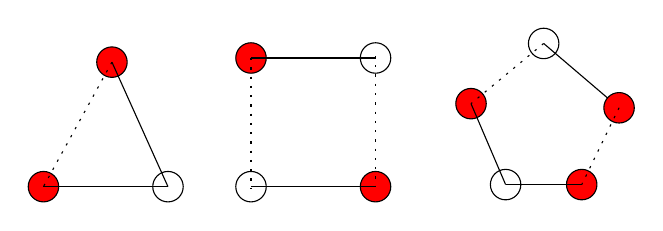
\begin{tikzpicture}[x=0.75pt,y=0.75pt,yscale=-1,xscale=1]
        %uncomment if require: \path (0,300); %set diagram left start at 0, and has height of 300

        %Shape: Circle [id:dp21271731455319154] 
        \draw   (274,59.33) .. controls (274,55.28) and (277.28,52) .. (281.33,52) .. controls (285.38,52) and (288.67,55.28) .. (288.67,59.33) .. controls (288.67,63.38) and (285.38,66.67) .. (281.33,66.67) .. controls (277.28,66.67) and (274,63.38) .. (274,59.33) -- cycle ;
        %Straight Lines [id:da3377214309921256] 
        \draw    (281.33,59.33) -- (317.67,90.33) ;
        %Shape: Circle [id:dp15239788247965558] 
        \draw  [fill={rgb, 255:red, 255; green, 0; blue, 0 }  ,fill opacity=1 ] (310.33,90.33) .. controls (310.33,86.28) and (313.62,83) .. (317.67,83) .. controls (321.72,83) and (325,86.28) .. (325,90.33) .. controls (325,94.38) and (321.72,97.67) .. (317.67,97.67) .. controls (313.62,97.67) and (310.33,94.38) .. (310.33,90.33) -- cycle ;
        %Shape: Circle [id:dp23851318758307316] 
        \draw  [fill={rgb, 255:red, 255; green, 0; blue, 0 }  ,fill opacity=1 ] (292.33,127.33) .. controls (292.33,123.28) and (295.62,120) .. (299.67,120) .. controls (303.72,120) and (307,123.28) .. (307,127.33) .. controls (307,131.38) and (303.72,134.67) .. (299.67,134.67) .. controls (295.62,134.67) and (292.33,131.38) .. (292.33,127.33) -- cycle ;
        %Shape: Circle [id:dp7542134009048679] 
        \draw   (255.67,127.33) .. controls (255.67,123.28) and (258.95,120) .. (263,120) .. controls (267.05,120) and (270.33,123.28) .. (270.33,127.33) .. controls (270.33,131.38) and (267.05,134.67) .. (263,134.67) .. controls (258.95,134.67) and (255.67,131.38) .. (255.67,127.33) -- cycle ;
        %Shape: Circle [id:dp2905682972946412] 
        \draw  [fill={rgb, 255:red, 254; green, 0; blue, 0 }  ,fill opacity=1 ] (239,88.33) .. controls (239,84.28) and (242.28,81) .. (246.33,81) .. controls (250.38,81) and (253.67,84.28) .. (253.67,88.33) .. controls (253.67,92.38) and (250.38,95.67) .. (246.33,95.67) .. controls (242.28,95.67) and (239,92.38) .. (239,88.33) -- cycle ;
        %Straight Lines [id:da5951249649317308] 
        \draw    (246.33,88.33) -- (263,127.33) ;
        %Straight Lines [id:da9315783025334317] 
        \draw  [dash pattern={on 0.84pt off 2.51pt}]  (281.33,59.33) -- (246.33,88.33) ;
        %Straight Lines [id:da5654511839083125] 
        \draw  [dash pattern={on 0.84pt off 2.51pt}]  (317.67,90.33) -- (299.67,127.33) ;
        %Straight Lines [id:da11049229477166267] 
        \draw    (299.67,127.33) -- (263,127.33) ;
        %Shape: Circle [id:dp13774885298457862] 
        \draw  [fill={rgb, 255:red, 255; green, 0; blue, 0 }  ,fill opacity=1 ] (193,128.33) .. controls (193,124.28) and (196.28,121) .. (200.33,121) .. controls (204.38,121) and (207.67,124.28) .. (207.67,128.33) .. controls (207.67,132.38) and (204.38,135.67) .. (200.33,135.67) .. controls (196.28,135.67) and (193,132.38) .. (193,128.33) -- cycle ;
        %Shape: Circle [id:dp6750434431270725] 
        \draw  [fill={rgb, 255:red, 255; green, 0; blue, 0 }  ,fill opacity=1 ] (133,66.33) .. controls (133,62.28) and (136.28,59) .. (140.33,59) .. controls (144.38,59) and (147.67,62.28) .. (147.67,66.33) .. controls (147.67,70.38) and (144.38,73.67) .. (140.33,73.67) .. controls (136.28,73.67) and (133,70.38) .. (133,66.33) -- cycle ;
        %Straight Lines [id:da5164768137625387] 
        \draw  [dash pattern={on 0.84pt off 2.51pt}]  (140.33,66.33) -- (140.33,129.33) ;
        %Shape: Circle [id:dp11262184380033369] 
        \draw   (133,128.33) .. controls (133,124.28) and (136.28,121) .. (140.33,121) .. controls (144.38,121) and (147.67,124.28) .. (147.67,128.33) .. controls (147.67,132.38) and (144.38,135.67) .. (140.33,135.67) .. controls (136.28,135.67) and (133,132.38) .. (133,128.33) -- cycle ;
        %Shape: Circle [id:dp1963388892901481] 
        \draw   (193,66.33) .. controls (193,62.28) and (196.28,59) .. (200.33,59) .. controls (204.38,59) and (207.67,62.28) .. (207.67,66.33) .. controls (207.67,70.38) and (204.38,73.67) .. (200.33,73.67) .. controls (196.28,73.67) and (193,70.38) .. (193,66.33) -- cycle ;
        %Straight Lines [id:da7532206160876841] 
        \draw  [dash pattern={on 0.84pt off 2.51pt}]  (200.33,65.33) -- (200.33,128.33) ;
        %Straight Lines [id:da9709146494537824] 
        \draw    (200.33,66.33) -- (140.33,66.33) ;
        %Straight Lines [id:da05709834301337491] 
        \draw    (200.33,128.33) -- (140.33,128.33) ;
        %Shape: Circle [id:dp47113483724287186] 
        \draw  [fill={rgb, 255:red, 255; green, 0; blue, 0 }  ,fill opacity=1 ] (66,68.33) .. controls (66,64.28) and (69.28,61) .. (73.33,61) .. controls (77.38,61) and (80.67,64.28) .. (80.67,68.33) .. controls (80.67,72.38) and (77.38,75.67) .. (73.33,75.67) .. controls (69.28,75.67) and (66,72.38) .. (66,68.33) -- cycle ;
        %Shape: Circle [id:dp22826385263304982] 
        \draw  [fill={rgb, 255:red, 255; green, 0; blue, 0 }  ,fill opacity=1 ] (33,128.33) .. controls (33,124.28) and (36.28,121) .. (40.33,121) .. controls (44.38,121) and (47.67,124.28) .. (47.67,128.33) .. controls (47.67,132.38) and (44.38,135.67) .. (40.33,135.67) .. controls (36.28,135.67) and (33,132.38) .. (33,128.33) -- cycle ;
        %Shape: Circle [id:dp43726961415276033] 
        \draw   (93,128.33) .. controls (93,124.28) and (96.28,121) .. (100.33,121) .. controls (104.38,121) and (107.67,124.28) .. (107.67,128.33) .. controls (107.67,132.38) and (104.38,135.67) .. (100.33,135.67) .. controls (96.28,135.67) and (93,132.38) .. (93,128.33) -- cycle ;
        %Straight Lines [id:da10952104956892128] 
        \draw  [dash pattern={on 0.84pt off 2.51pt}]  (73.33,68.33) -- (40.33,128.33) ;
        %Straight Lines [id:da548029525751494] 
        \draw    (73.33,68.33) -- (100.33,128.33) ;
        %Straight Lines [id:da5236546881149744] 
        \draw    (40.33,128.33) -- (100.33,128.33) ;




    \end{tikzpicture}

\end{figure}
It is easy to see that
\begin{align*}
    |\text{maximum matching of }C_n|
     & =\left\lfloor \frac{n}{2} \right\rfloor \\
     & \left( =
    \begin{cases}
            \frac{n}{2}   & n \text{ even} \\
            \frac{n-1}{2} & n \text{ odd}
        \end{cases}\right)
\end{align*}
For even cycles, (every other vertex) is a cover of size $ \frac{n}{2} $, so
is a minimum cover by~\ref{equality cover}.
For odd cycles, the minimum cover has size $ \lceil \frac{n}{2} \rceil $
because $ \lfloor \frac{n}{2} \rfloor  $ is not enough since every vertex has
degree $ 2 $.

So, for $ C_n $,
\[ |\text{maximum matching of }C_n|=\left\lfloor \frac{n}{2} \right\rfloor \]
\[ |\text{minimum cover of }C_n|=\left\lceil \frac{n}{2} \right\rceil \]
Therefore, $ |\text{maximum matching}|=|\text{minimum cover}| $ if and only if
$ n $ is even; that is, $ C_n $ is bipartite.

\underline{Paths}: Let $ P_n $ be a path on $ n $ vertices. We take
every other edge to be in the maximum matching.

\begin{figure}[H]
    \centering
    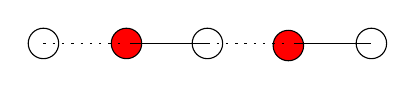
\begin{tikzpicture}[x=0.75pt,y=0.75pt,yscale=-1,xscale=1]
        %uncomment if require: \path (0,300); %set diagram left start at 0, and has height of 300

        %Shape: Circle [id:dp5638841377720051] 
        \draw  [fill={rgb, 255:red, 255; green, 0; blue, 0 }  ,fill opacity=1 ] (195,80.33) .. controls (195,76.28) and (198.28,73) .. (202.33,73) .. controls (206.38,73) and (209.67,76.28) .. (209.67,80.33) .. controls (209.67,84.38) and (206.38,87.67) .. (202.33,87.67) .. controls (198.28,87.67) and (195,84.38) .. (195,80.33) -- cycle ;
        %Shape: Circle [id:dp3041773169214014] 
        \draw   (155,80.33) .. controls (155,76.28) and (158.28,73) .. (162.33,73) .. controls (166.38,73) and (169.67,76.28) .. (169.67,80.33) .. controls (169.67,84.38) and (166.38,87.67) .. (162.33,87.67) .. controls (158.28,87.67) and (155,84.38) .. (155,80.33) -- cycle ;
        %Straight Lines [id:da3693432195767684] 
        \draw  [dash pattern={on 0.84pt off 2.51pt}]  (162.33,80.33) -- (202.33,80.33) ;
        %Straight Lines [id:da3569703809119109] 
        \draw    (204,80.33) -- (241.33,80.33) ;
        %Shape: Circle [id:dp24958723200717514] 
        \draw   (234,80.33) .. controls (234,76.28) and (237.28,73) .. (241.33,73) .. controls (245.38,73) and (248.67,76.28) .. (248.67,80.33) .. controls (248.67,84.38) and (245.38,87.67) .. (241.33,87.67) .. controls (237.28,87.67) and (234,84.38) .. (234,80.33) -- cycle ;
        %Shape: Circle [id:dp1744775588707035] 
        \draw   (313,80.33) .. controls (313,76.28) and (316.28,73) .. (320.33,73) .. controls (324.38,73) and (327.67,76.28) .. (327.67,80.33) .. controls (327.67,84.38) and (324.38,87.67) .. (320.33,87.67) .. controls (316.28,87.67) and (313,84.38) .. (313,80.33) -- cycle ;
        %Shape: Circle [id:dp6522716415155324] 
        \draw  [fill={rgb, 255:red, 255; green, 0; blue, 0 }  ,fill opacity=1 ] (273,81.33) .. controls (273,77.28) and (276.28,74) .. (280.33,74) .. controls (284.38,74) and (287.67,77.28) .. (287.67,81.33) .. controls (287.67,85.38) and (284.38,88.67) .. (280.33,88.67) .. controls (276.28,88.67) and (273,85.38) .. (273,81.33) -- cycle ;
        %Straight Lines [id:da18775481471991495] 
        \draw  [dash pattern={on 0.84pt off 2.51pt}]  (241.33,80.33) -- (281.33,80.33) ;
        %Straight Lines [id:da08079748979020784] 
        \draw    (283,80.33) -- (320.33,80.33) ;
    \end{tikzpicture}
    \caption{$ P_5 $}
\end{figure}

\begin{figure}[H]
    \centering
    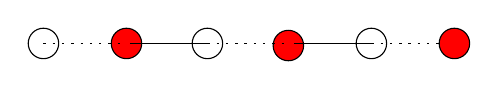
\begin{tikzpicture}[x=0.75pt,y=0.75pt,yscale=-1,xscale=1]
        %uncomment if require: \path (0,300); %set diagram left start at 0, and has height of 300

        %Shape: Circle [id:dp5638841377720051] 
        \draw  [fill={rgb, 255:red, 255; green, 0; blue, 0 }  ,fill opacity=1 ] (195,80.33) .. controls (195,76.28) and (198.28,73) .. (202.33,73) .. controls (206.38,73) and (209.67,76.28) .. (209.67,80.33) .. controls (209.67,84.38) and (206.38,87.67) .. (202.33,87.67) .. controls (198.28,87.67) and (195,84.38) .. (195,80.33) -- cycle ;
        %Shape: Circle [id:dp3041773169214014] 
        \draw   (155,80.33) .. controls (155,76.28) and (158.28,73) .. (162.33,73) .. controls (166.38,73) and (169.67,76.28) .. (169.67,80.33) .. controls (169.67,84.38) and (166.38,87.67) .. (162.33,87.67) .. controls (158.28,87.67) and (155,84.38) .. (155,80.33) -- cycle ;
        %Straight Lines [id:da3693432195767684] 
        \draw  [dash pattern={on 0.84pt off 2.51pt}]  (162.33,80.33) -- (202.33,80.33) ;
        %Straight Lines [id:da3569703809119109] 
        \draw    (204,80.33) -- (241.33,80.33) ;
        %Shape: Circle [id:dp24958723200717514] 
        \draw   (234,80.33) .. controls (234,76.28) and (237.28,73) .. (241.33,73) .. controls (245.38,73) and (248.67,76.28) .. (248.67,80.33) .. controls (248.67,84.38) and (245.38,87.67) .. (241.33,87.67) .. controls (237.28,87.67) and (234,84.38) .. (234,80.33) -- cycle ;
        %Shape: Circle [id:dp1744775588707035] 
        \draw   (313,80.33) .. controls (313,76.28) and (316.28,73) .. (320.33,73) .. controls (324.38,73) and (327.67,76.28) .. (327.67,80.33) .. controls (327.67,84.38) and (324.38,87.67) .. (320.33,87.67) .. controls (316.28,87.67) and (313,84.38) .. (313,80.33) -- cycle ;
        %Shape: Circle [id:dp6522716415155324] 
        \draw  [fill={rgb, 255:red, 255; green, 0; blue, 0 }  ,fill opacity=1 ] (273,81.33) .. controls (273,77.28) and (276.28,74) .. (280.33,74) .. controls (284.38,74) and (287.67,77.28) .. (287.67,81.33) .. controls (287.67,85.38) and (284.38,88.67) .. (280.33,88.67) .. controls (276.28,88.67) and (273,85.38) .. (273,81.33) -- cycle ;
        %Straight Lines [id:da18775481471991495] 
        \draw  [dash pattern={on 0.84pt off 2.51pt}]  (241.33,80.33) -- (281.33,80.33) ;
        %Straight Lines [id:da08079748979020784] 
        \draw    (283,80.33) -- (320.33,80.33) ;
        %Straight Lines [id:da6611106612682713] 
        \draw  [dash pattern={on 0.84pt off 2.51pt}]  (320.33,80.33) -- (344.33,80.33) -- (360.33,80.33) ;
        %Shape: Circle [id:dp2871716009686791] 
        \draw  [fill={rgb, 255:red, 255; green, 0; blue, 0 }  ,fill opacity=1 ] (353,80.33) .. controls (353,76.28) and (356.28,73) .. (360.33,73) .. controls (364.38,73) and (367.67,76.28) .. (367.67,80.33) .. controls (367.67,84.38) and (364.38,87.67) .. (360.33,87.67) .. controls (356.28,87.67) and (353,84.38) .. (353,80.33) -- cycle ;
    \end{tikzpicture}
    \caption{$ P_6 $}
\end{figure}

It is easy to check that
\[ |\text{maximum matching of }P_n|=\left\lfloor \frac{n}{2} \right\rfloor \]
\[ |\text{minimum cover of }P_n|=\left\lfloor \frac{n}{2} \right\rfloor \]
Thus,
\[ |\text{maximum matching of }P_n|=|\text{minimum cover of }P_n| \]

It follows that, if $ G $ is a bipartite graph where every component is a path or cycle,
then
\[ |\text{maximum matching of }G|=|\text{minimum cover of }G|  \]
\begin{proof}
    A maximum matching of $ G $ consists of a maximum matching for each component. Same for
    the minimum cover. Since we know $ |\text{maximum matching}|=|\text{minimum cover}| $
    for each component, the same is true for $ G $.
\end{proof}

\begin{thmbox}
    \begin{prop}
        Let $ G $ be a graph with no vertices of degree $ 3 $ or more. Then
        every component of $ G $ is a path or cycle.
    \end{prop}
\end{thmbox}
\begin{proof}
    Let $ C $ be a component of $ G $. Let $ P $ be a longest path
    in $ C $. Let $ u $ and $ v $ be the ends of $ P $. Since every vertex
    of $ P $ has degree $ \geqslant 2 $, the only possible edge in $ C $ that is
    not in $ P $ is the edge from $ u $ to $ v $. Therefore, either
    $ P=C $, or $ C $ is a cycle. So every component is a path or cycle.
\end{proof}

\begin{thmbox}
    \begin{prop}\label{equality matching}
        If $ M $ is a matching of $ G $ and $ C $ is a cover of $ G $ with $ |M|=|C| $,
        then every vertex in $ C $ is the end of an edge in $ M $.
    \end{prop}
\end{thmbox}
\begin{proof}
    Since $ C $ is a cover, every edge in $ M $ has an end in $ C $; since $ M $
    is a matching, these ends are all different, so there is nothing else in $ C $.
\end{proof}
We can now prove~\ref{konig}.
\begin{thmbox}
    \begin{theorem}[König's Theorem (1931)]
        If $ G $ is a bipartite graph, then
        \[ |\text{maximum matching of }G|=|\text{minimum cover of }G| \]
    \end{theorem}
\end{thmbox}
The proof in course notes is longer since it is used for the algorithm:
a maximum matching in a bipartite graph, that is usually within this course,
but due to the lack of time, we will not present it here, and hence the proof presented
will be different.
\begin{proof}
    Rizzi (1999). We use strong induction.
    The theorem is obvious for graphs with no edges; let $ G $
    be a bipartite graph with $ m>0 $ edges, and suppose that the theorem holds
    for every bipartite graph with $ <m $ edges. Let $ k $ be the size of a
    maximum matching. If every vertex of $ G $ has degree $ \leqslant 2 $, then every
    component is a path or cycle, so König's Theorem holds. Let $ u $ be a vertex of
    $ G $ of degree $ \geqslant 3 $, and let $ v $ be a neighbour of $ u $.

    \underline{Case 1}: The graph $ G-v $ has no matching of size $ k $. If this is true,
    the graph $ G-v $ has a maximum matching if size $ \leqslant k-1 $. Since $ G-v $
    is bipartite and has fewer edges than $ G $, the inductive hypothesis implies that
    $ G-v $ has a cover $ C_1 $ of size $ \leqslant k-1 $. So $ C_1\cup \{v\} $
    is a cover of $ G $ of size $ \leqslant k $. Since $ k $ is the size of a matching of
    $ G $, we have $ |C_1\cup \{v\}|\geqslant k $, so $ C_1 \cup \{v\} $ is a cover
    of the same size as a matching of $ G $, so by~\ref{equality matching},
    we have
    \[ |\text{maximum matching}|=|\text{minimum cover}| \]
    \underline{Case 2}: The graph $ G-v $ does have a matching of size $ k $. Let
    $ M $ be such a matching; that is, $ |M|=k $ and $ M $ does not saturate $ v $.
    Let $ f $ be an edge not in $ M $, that is incident with $ u $ but not $ v $.
    Since $ G-f $ is bipartite and has fewer edges than $ G $, and has a matching $ M $
    of size $ k $, inductively $ G-f $ has a cover $ C_2 $ of size $ k $. Since
    $ |C_2|=|M| $ every vertex in $ C_2 $ is saturated by $ M $ by~\ref{equality matching},
    so $ v\notin C_2 $. Since $ C_2 $ contains $ \geqslant 1 $ end of the edge $ uv $,
    we have $ u\in C_2 $. So, $ C_2 $ contains an end of $ f $, and an end of every edge in
    $ G-f $. So $ C_2 $ is a cover of $ G $ of size $ k = |\text{maximum matching}| $.
    So $ C_2 $ is a minimum cover; thus
    \[ |\text{maximum matching}|=|\text{minimum cover}| \]
\end{proof}
